\documentclass[11pt,a4paper]{article}
\usepackage[margin=19mm,top=20mm,bottom=20mm]{geometry}
\usepackage{amsmath,amssymb,graphicx,array,fancyhdr,lastpage,textcomp,fancyvrb}
\usepackage{fontspec}
\usepackage[hidelinks]{hyperref}
\setmainfont{texgyreheros-regular.otf}[BoldFont=texgyreheros-bold.otf,ItalicFont=texgyreheros-italic.otf,BoldItalicFont=texgyreheros-bolditalic.otf]
\setmonofont{lmmono10-regular.otf}
\setlength{\parindent}{0pt}\setlength{\parskip}{5pt}
\setlength{\headheight}{14pt}
\pagestyle{fancy}\fancyhf{}
\renewcommand{\headrulewidth}{0.3pt}\renewcommand{\footrulewidth}{0.3pt}
\fancyfoot[L]{\footnotesize by paper.shrit.in\quad |\quad normal}
\fancyfoot[R]{\footnotesize Page \thepage\ of \pageref{LastPage}}
\begin{document}
\fancyhead[L]{\small Data Communication and Computer Networks}\fancyhead[R]{\small Set B: Original}
{\LARGE\bfseries Worked Solutions}\par{\large Data Communication and Computer Networks}\par\textbf{Set B: Original | CSE Semester 3}\par
Companion to \texttt{dccn-original.pdf}. Question numbers match that paper. Equivalent correct methods are acceptable. These are independent worked solutions, not an official university marking scheme.\par\medskip\hrule\medskip
Questions 1--5: MCQ answer key, 1 mark each (5 marks total). Questions 6 onward: theory solutions (25 marks total).\par
\noindent\begin{minipage}{\linewidth}\subsection*{1. Nyquist rate}
\textbf{Correct option: (C).} $R=2B\log_2L=2(3000)\log_2 4=12000$ bps.
\end{minipage}\par\medskip
\noindent\begin{minipage}{\linewidth}\subsection*{2. Bits per symbol}
\textbf{Correct option: (B).} Four levels represent $\log_2 4=2$ bits per symbol.
\end{minipage}\par\medskip
\noindent\begin{minipage}{\linewidth}\subsection*{3. Shannon capacity}
\textbf{Correct option: (A).} $C=B\log_2(1+S/N)=3000\log_2 32=15000$ bps.
\end{minipage}\par\medskip
\noindent\begin{minipage}{\linewidth}\subsection*{4. Tighter rate bound}
\textbf{Correct option: (D).} Both limits must hold, so the smaller upper bound, 12 kbps, is tighter.
\end{minipage}\par\medskip
\noindent\begin{minipage}{\linewidth}\subsection*{5. Nyquist bandwidth change}
\textbf{Correct option: (C).} $R=2B\log_2L$ is directly proportional to $B$ when $L$ is fixed.
\end{minipage}\par\medskip
\noindent\begin{minipage}{\linewidth}\subsection*{6. Modulation comparison}

ASK changes carrier amplitude, FSK changes carrier frequency, and PSK changes carrier phase. Binary FSK commonly uses two separated frequencies and needs more bandwidth than binary PSK under comparable simple pulse shaping. ASK and BPSK can have comparable nominal bandwidth for the same bit rate and shaping; exact occupied bandwidth depends on the implementation. ASK is directly vulnerable to amplitude disturbances. Constant-envelope FSK and PSK are less affected by such disturbances, although phase/frequency noise and receiver synchronization still matter.

For a coherent receiver in an approximately additive-noise, bandwidth-limited telephone channel, BPSK is a defensible choice: it uses antipodal signals, offers good bit-error performance at a given energy per bit, and avoids the tone separation of binary FSK. A noncoherent, very simple receiver could instead favor FSK. The noise model and implementation must be stated rather than claiming one scheme is always best.
\end{minipage}\par\medskip
\noindent\begin{minipage}{\linewidth}\subsection*{7. Header overhead}

Header bytes $=5(20)=100$. Total bytes $=900+100=\boxed{1000}$.
Header percentage $=100/1000\times100=\boxed{10\%}$. Payload efficiency is 90\%.
\end{minipage}\par\medskip
\noindent\begin{minipage}{\linewidth}\subsection*{8. CRC division and receiver check}

Append four zeros because the generator 10011 has degree four. The aligned XOR working dividends are:
\begin{verbatim}
11010110110000  initial dividend
01001110110000
00000010110000
00000000101000
00000000001110
\end{verbatim}
The remainder is $\boxed{1110}$ and the transmitted codeword is $\boxed{11010110111110}$. The receiver divides the whole received codeword by 10011. A zero remainder means no error was detected; it does not guarantee that no undetectable error occurred.
\end{minipage}\par\medskip
\noindent\begin{minipage}{\linewidth}\subsection*{9. Manchester and AMI waveforms}
Manchester half-bit pairs are $(-,+),(+,-),(-,+),(-,+),(+,-),(+,-),(-,+),(+,-)$. AMI levels are $+,0,-,+,0,0,-,0$. These use the conventions printed in the question.\begin{center}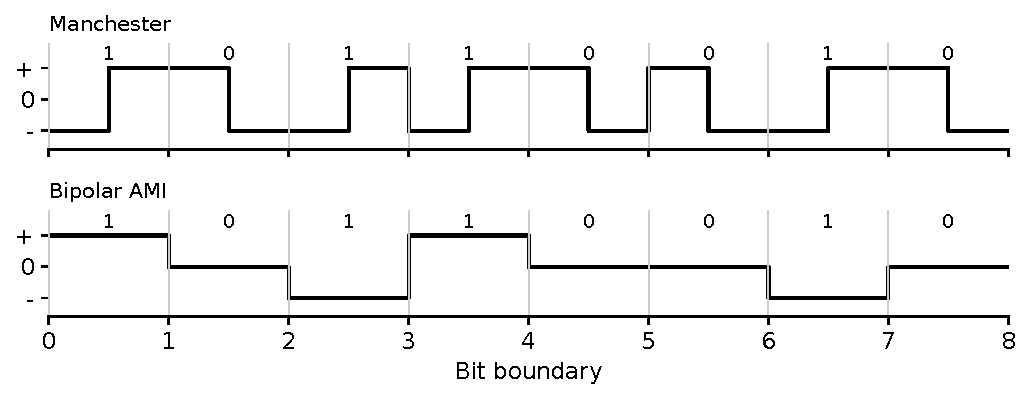
\includegraphics[width=.85\linewidth]{figures/line-original.pdf}\end{center}
\end{minipage}\par\medskip
\noindent\begin{minipage}{\linewidth}\subsection*{10. Hub and learning switch}
A hub repeats the incoming physical signal on every other port. A learning switch records source MAC to ingress-port mappings. For a known destination on a different port, it forwards only there; for a known destination on the incoming port, it filters the frame. For an unknown destination it floods on other forwarding ports in the same VLAN. Broadcasts are also flooded within that VLAN.
\end{minipage}\par\medskip
\noindent\begin{minipage}{\linewidth}\subsection*{11. Stop-and-wait throughput}

Frame length $L=1000(8)=8000$ bits. Serialization time:
\[t_t=8000/10^6=\boxed{8\ \mathrm{ms}}.\]
Cycle time from starting a frame until its ACK returns:
\[t_{cycle}=t_t+2t_p=8+20=\boxed{28\ \mathrm{ms}}.\]
\[U=\frac8{28}=\boxed{0.285714},\qquad
\mathrm{throughput}=\frac{8000}{0.028}=\boxed{285714.3\ \mathrm{bps}}.\]
Thus utilization is 28.57\% and useful throughput is approximately 285.7 kbps. There are no headers or losses in this calculation.
\end{minipage}\par\medskip
\noindent\begin{minipage}{\linewidth}\subsection*{12. Selective repeat versus go-back-N}

Selective repeat accepts frame 0 and buffers frames 2 and 3 while waiting for 1. Only frame 1 remains unacknowledged and is retransmitted. After it arrives, the receiver delivers 1, 2 and 3, giving overall delivery order $0,1,2,3$. There are five data transmissions in total.

Go-back-N accepts 0, discards 2 and 3, and uses cumulative acknowledgements. After frame 1 times out, it retransmits the outstanding suffix 1, 2 and 3. There are seven data transmissions in total and the same final delivery order.
\end{minipage}\par\medskip
\noindent\begin{minipage}{\linewidth}\subsection*{13. Minimum collision-detection frame}

\[L_{\min}=R(2t_p)=100\times10^6\times10\times10^{-6}
=\boxed{1000\ \mathrm{bits}=125\ \mathrm{bytes}}.\]
This is the propagation-only lower bound for the hypothetical link in the question.
\end{minipage}\par\medskip

\end{document}
